\usetikzlibrary{patterns}
\usetikzlibrary{decorations.pathmorphing}
\usepackage{titlesec,calc}
% \renewcommand{\familydefault}{\sfdefault}

\titleformat{\section}[hang]
{\normalfont\bfseries}
{\thesection.}{0.5em}{}
 \titlespacing{\section}{0pt}{3pt}{2pt} % Horizontal space, before space, after space

\mode<presentation>
{
  \usetheme{CambridgeUS}
  \usecolortheme{whale}
  \usecolortheme{lily}

  \setbeamercovered{transparent}
  \usefonttheme[onlymath]{serif}
}

\title[Simulation] % (optional, use only with long paper titles)
{\large \course: \coursename \\[5pt] \semesteryear\\[5pt] Exercise 2: System Simulation}

\subtitle
{} % (optional)

\author[\instructorshort]% (optional, use only with lots of authors)
{\instructorlong\credits}
%{T. Vincent\inst{1} \and S.~Another\inst{2}}
% - Use the \inst{?} command only if the authors have different
%   affiliation.

\institute[\instituteshort] % (optional, but mostly needed)
{\institutelong}


\date % (optional)
{}



% If you have a file called "university-logo-filename.xxx", where xxx
% is a graphic format that can be processed by latex or pdflatex,
% resp., then you can add a logo as follows:

%\pgfdeclareimage[height=1.1cm]{university-logo}{UniversityLogo}
%\logo{\pgfuseimage{university-logo}}



% Delete this, if you do not want the table of contents to pop up at
% the beginning of each subsection:
%\AtBeginSection[]
%{
%  \begin{frame}<beamer>{Outline}
%    \tableofcontents[currentsection,currentsubsection]
%  \end{frame}
%}


% If you wish to uncover everything in a step-wise fashion, uncomment
% the following command:

%\beamerdefaultoverlayspecification{<+->}


\begin{document}



\begin{frame}
  \titlepage
\end{frame}

\mode<article>{
\maketitle
%\tableofcontents
}

%\mode<presentation>{
%\begin{frame}{Outline}
%  \tableofcontents
%  % You might wish to add the option [pausesections]
%\end{frame}}

\section{Introduction}
The purpose of this exercise is to create a simulation of a vehicle using \textsc{Matlab} and Simulink. 

\section{Simulink Introduction}

You will need to learn how to enter and simulate differential equations in Simulink. You should do this {\em before} coming to lab. The following resources may be useful:
\begin{itemize}
\item Simulink video tutorials: \url{http://www.mathworks.com/academia/student_center/Tutorials/simulink-launchpad.html} (Suggest viewing Simulink On-Ramp and Using Simulink to Model Continuous Dynamical Systems)
\item Michigan/CMU Simulink Tutorial: \url{http://ctms.engin.umich.edu/CTMS/index.php?example=Introduction&section=SimulinkModeling}
\end{itemize}
Note that you can get access to Matlab and Simulink at most any computer lab on campus, and in addition, you can utilize the virtual lab at \url{matlab.mines.edu}. It is expected that you are already familiar with \textsc{Matlab} and creating \textsc{Matlab} functions. If not, you may also want to look at the Mathworks tutorials for \textsc{Matlab}.

\section{The System}

The vehicle to be simulated is shown in cartoon form below. It has wheels which are driven by a motor.  The position of the vehicle is measured relative to an (arbitrary) fixed point, with horizontal location $x$ and vertical location $y$. (We assume the vehicle moves in a straight line, so only two axes are necessary).  The vehicle drives along a road with road surface height given by the function $r(x)$. 

%\begin{figure}
\begin{center}
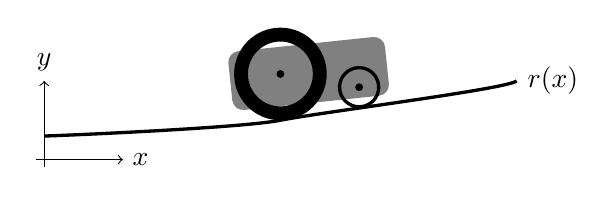
\begin{tikzpicture}[very thick,
sysblock/.style={draw,rectangle,inner sep=6pt,minimum width=1.5cm,minimum height=1.2cm,very thick},
delayblock/.style={draw,rectangle,inner sep=6pt,minimum width=0.5cm,minimum height=1.0cm,very thick},
node/.style={fill,inner sep=0pt,outer sep=0pt},
summer/.style={circle,draw,very thick,inner sep=5pt}]

\draw (0,.3) .. controls +(.11,0) and +(-.5,-.1) .. (3,.5) .. controls +(.5,.1) and +(-.1,-.1) .. (6,1) node[right] {$r(x)$}; 
\draw[->,thin] (-.1,0) -- (1,0) node[right] {$x$}; 
\draw[->,thin] (0,-.1) -- (0,1) node[above] {$y$}; 
\draw (3.4,.7) node[rotate=6,above,fill=gray,rectangle,minimum width=2cm, minimum height=0.75cm,rounded corners] (M) {};
\draw (3,.5) node[summer,above,minimum height=1cm,line width=5pt] (W1) {};
\draw (W1) node[circle,fill=black,inner sep=0pt,outer sep=0pt,minimum height=.1cm] {};
\draw (4,.65) node[summer,above] (W2) {};
\draw (W2) node[circle,fill=black,inner sep=0pt,outer sep=0pt,minimum height=.1cm] {};


\end{tikzpicture}

\end{center}

The differential equation that describes the movement of the vehicle in the $x$ direction is given by 
\[
\boxed{\ddot{x} = \cos(\phi)\left[ -\frac{d^2r}{dx^{2}}(\dot{x})^2\sin(\phi) - g\sin(\phi) + \frac{1}{m}f - \frac{b}{m\cos(\phi)}\dot{x}\right]}.
\]
The  parameters in this equation are the following:
\begin{center}
\begin{tabular}{l|l}
Parameter & Description\\\hline
$f$ & force on the vehicle due to motor/tires (N)\\
$g$ & gravitational accelleration 9.81 m/s$^2$\\
$m$ & mass of the vehicle (kg)\\
$b$ & translational drag constant (Ns/m)\\
$\phi = \tan^{-1}(\frac{dr}{dx})$ & the angle that the road makes with the horizontal (rad)\\
\end{tabular}
\end{center}
The assumptions behind and derivation of this equation can be found in the Appendix. 

You will use Simulink to solve this differential equation. Once you find $x(t)$, $y(t)$ is given by $y(t)=r(x(t))$.

\section{Creating your road}

To implement the simulation, you will need a function to return various characteristics of the road at location $x$, specifically $r(x)$, $\phi = \tan^{1}\left(\frac{dr}{dx}\right)$ and $\frac{d^2r}{dx^2}$. If you define $r(x)$ first, you run the risk of creating a function that is not differentiable twice. Thus, it is easier to define $\frac{d^2r}{dx^2}$ first, and then integrate twice to get the other functions. The following \textsc{Matlab} function is an example of using this approach. Note that the line \texttt{cumsum(ddr)*dx} is a cumulative sum that implements a discrete approximation of the integral. Type \texttt{help cumsum} for more information.

\begin{alltt}
%
% Grid on which to define d^2r/dx^2
%
dx=.1;
x = 0:dx:10; \% m
%
% Initialize d^2r/dx^2 as zero
%
ddr = zeros(size(x));
%
% Increasing slope between 1 m and 1.5 m
% To end at a slope of 1/3, magnitude of d^2r/dx^2 = (1/3)/0.5
%
index = find(x>=1 & x<1.5);
ddr(index) = ((1/3)/0.5)*ones(size(index));
%
% Decreasing slope between 7 m and 8 m
% want to end back a slope of 0
%
index = find(x>=7 & x<8);
ddr(index) = -((1/3)/1)*ones(size(index));
%
% Find dr/dx, phi, and r
%
dr = cumsum(ddr)*dx;
phi = atan(dr);
r = cumsum(dr)*dx;
%
% Plot the results
%
figure(1)
clf
set(gca,\T\hspace{0pt}fontsize\T,16) \% make sure text is readable
subplot(3,1,1)
plot(x,ddr)
subplot(3,1,2)
plot(x,dr)
ylabel(\T\$\textbackslash\hspace{0pt}frac\{d r\}\{dx\}\$\T,\T\hspace{0pt}interpreter\T,\T\hspace{0pt}latex\T)
subplot(3,1,3)
plot(x,r)
ylabel(\T\$r\$\T,\T\hspace{0pt}interpreter\T,\T\hspace{0pt}latex\T)
xlabel(\T\$x\$ (m)\T,\T\hspace{0pt}interpreter\T,\T\hspace{0pt}latex\T)
%
% Save the results in a .mat file
%
save road.mat x r dr ddr phi


\end{alltt}


\section{Deliverables}
\begin{itemize}
\item Implement a simulation of the vehicle model in Simulink. Because the equations are fairly complicated, the  \textsf{Matlab function} block, found in the User-Defined Functions library, could be useful. (Use the \textsc{Matlab} help to get more information on how to use this block.) In addition, you will want to use a \textsf{1-D lookup table} block, found in the Lookup Tables library, to implement $r(x)$, $\phi(x)$, and $\frac{d^2 r}{dx^2}(x)$. If the results of the above script are in the local workspace, then setting \textsf{Breakpoints 1:} to \textsf{x} and \textsf{Table Data:} to \textsf{r}, \textsf{phi}, or \textsf{ddr}, as appropriate, will implement a linear interpolation of the road data.  Implement your simulation so that the parameters (i.e. $m$, $b$, etc.) are easy to change.  The following example shows a typical configuration
\begin{center}
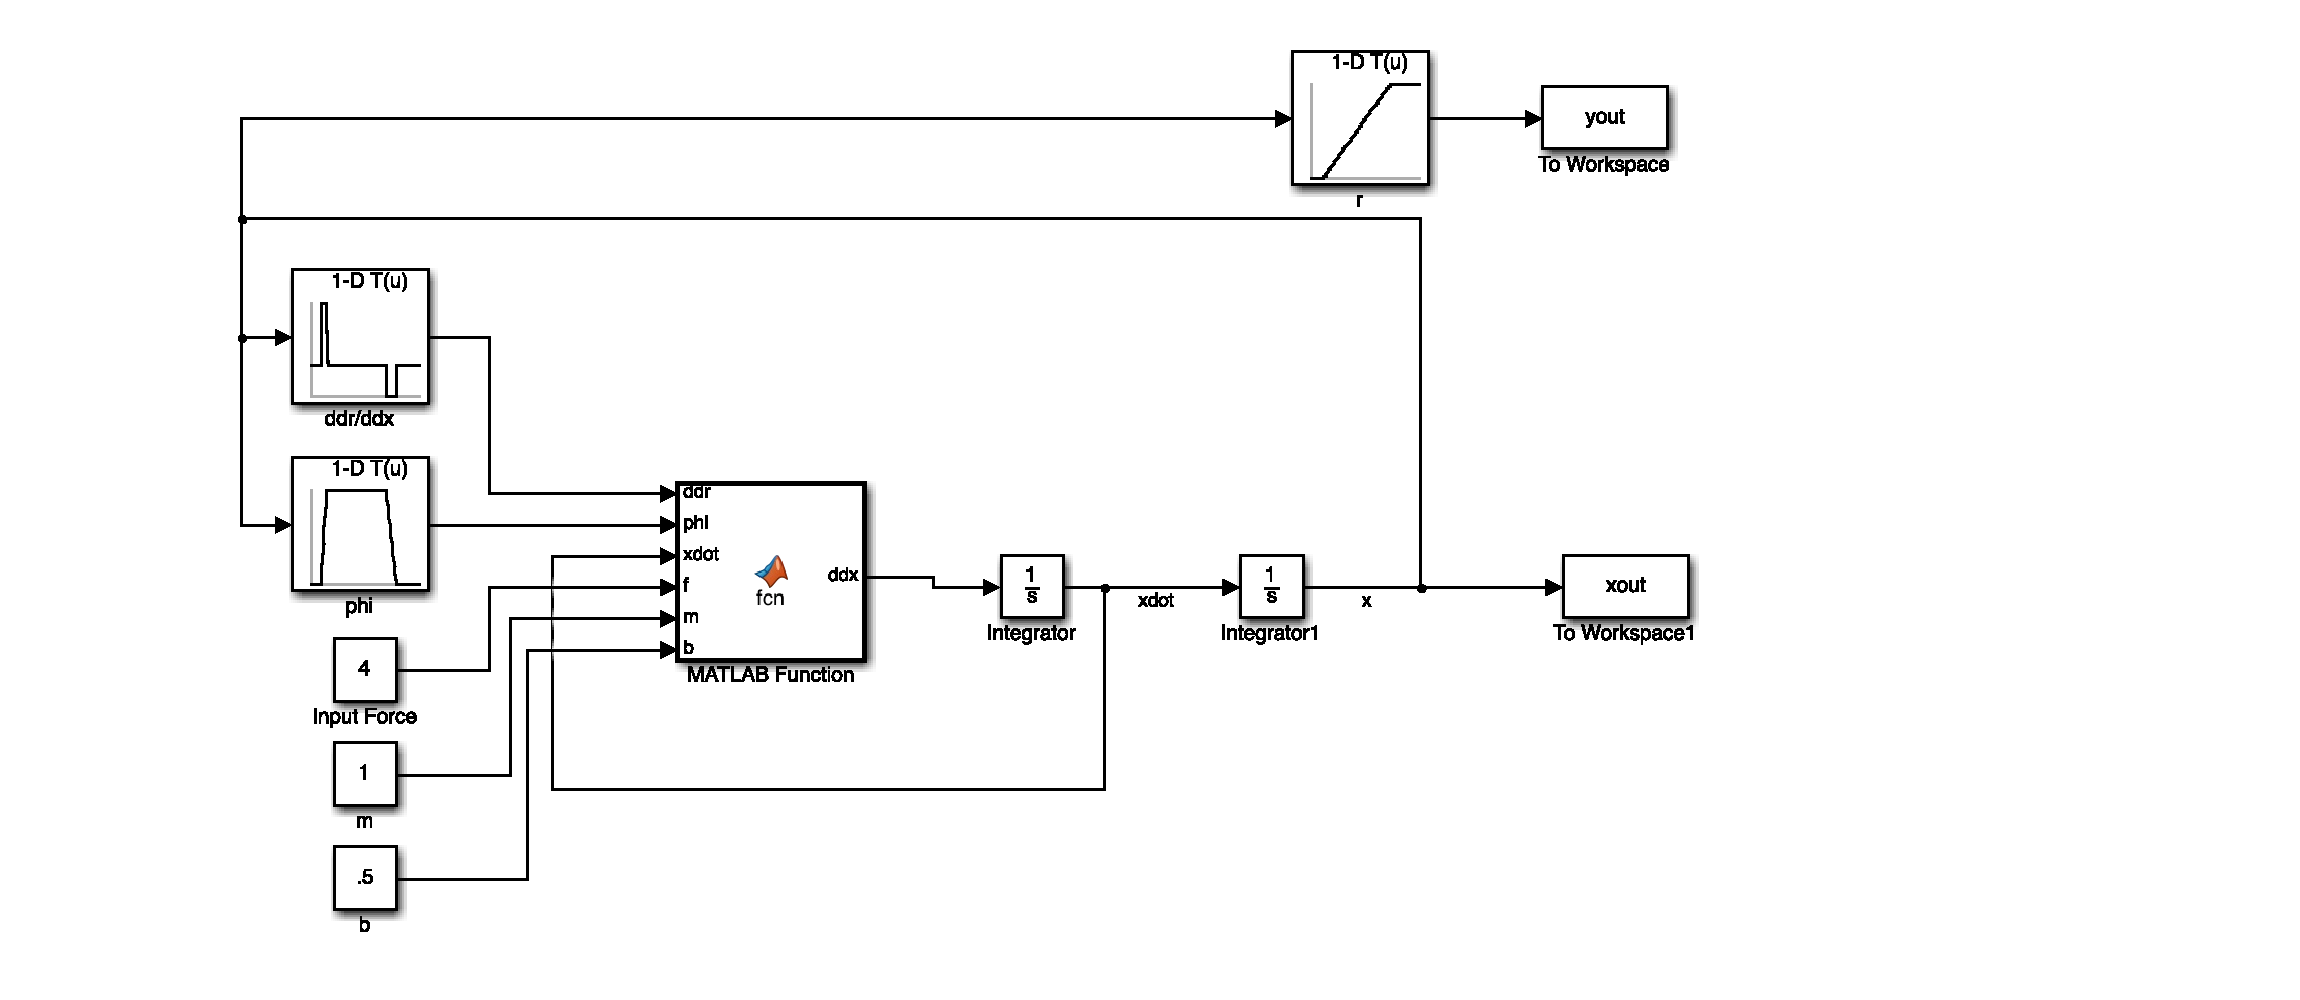
\includegraphics[width=6in]{Graphics/blockdiag}
\end{center}
Note that \textsf{to workspace} blocks are used to save the results in the variables \textsf{yout} and \textsf{xout}. The default is for these variables to be structures called Timeseries. After running the simulation, type the name of the variable (i.e. \textsf{yout}) at the command line to see the elements of the structure. \textsf{yout.Data} will give you access to the data, while \textsf{yout.Time} to the corresponding time points. However, the \textsf{plot} command will recognize a Timeseries, so you can just type \textsf{plot(yout)} to get a plot of $y$ verses time.
\item Create an animation that shows the results of the simulations.
\begin{itemize}
\item Click on the Matlab Help (located on the home tab of the command window), then click on \textsf{Matlab}, \textsf{Graphics}, \textsf{2-D and 3-D Plots}, and \textsf{Animation}. Try each of the ``Examples and How To''.
\item This link gives a detailed example of an animation, and the example of animating a bouncing ball is very close to animating the motion of the vehicle. \url{https://zerocrossraptor.wordpress.com/matlab-undercover/creating-simple-animation-in-matlab/}
\end{itemize}
\item Re-read the EENG307 lecture notes on PID control, posted on the blackboard site. In simulink, implement a PI controller to regulate the speed of the robot, assuming that you can directly control the applied force $f$. Use the linearized system dynamics 
\[
\ddot{x} + \frac{b}{m}\dot{x} = \frac{1}{m}f.
\]
as the design model. These dynamics assume a flat road, but the I term in your controller should help account for the force due to a non-flat road. Show that the controller regulates the speed even as the road slope varies.
\item Create a document that discusses the results of your Simulink simulation, with enough detail that someone else could recreate the results. This document should include the Simulink block digram, system and simulation parameters, plots of the results, and an interpretation of the results.
\item Store your simulink model and animation code for future use.
\end{itemize}

\section{Demonstrations}
\begin{itemize}
\item Be prepared to demonstrate your simulation and animation.
\end{itemize}

\section{Appendix: Vehicle Model}
To model this system, we have to decide what detail we would like to include. For this exercise, lets model the robot as a single mass of $m$ kg, ignoring rotational effects (including the interia in the rotating tires). When the motor spins the tires, (assuming they don't slip) a force of $f$ N is applied to the mass. Due to wind or other friction forces, a damping force of $f_{d}=b\dot{v}$ N acts against the vehicle motion, where $\dot{v}$ is the vehicle velocity. The angle of the road at the location of the vehicle is $\phi$. This simplified model is shown below, to the left. The road surface supports the vehicle with contact force $f_{c}$, and gravity exerts a force of $mg$ N, where $g$ is gravitational accleration. The the free body diagram is shown below, to the right.
\begin{center}
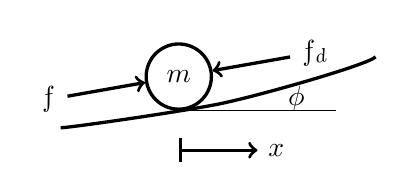
\begin{tikzpicture}[very thick,
sysblock/.style={draw,rectangle,inner sep=6pt,minimum width=1.5cm,minimum height=1.2cm,very thick},
delayblock/.style={draw,rectangle,inner sep=6pt,minimum width=0.5cm,minimum height=1.0cm,very thick},
node/.style={fill,inner sep=0pt,outer sep=0pt},
summer/.style={circle,draw,very thick,inner sep=5pt}]

\draw (0,0) node[summer] (M1) {$m$};

\draw[thin]  (M1.-90) -- ++(2,0);
\draw (M1.-90) ++(6:1.5) node {$\phi$};
\draw[|->] (M1.-90) ++(0,-.5) -- ++(1,0) node[right] {$x$};
\draw (-1.5,-.65) .. controls +(.11,0) and +(-.5,-.1) .. ++(2,.3) .. controls +(.5,.1) and +(-.1,-.1) .. ++(2,.6);
\draw[->] (M1.190) ++(10:-1) node[rotate=10,left] {$f$} -- (M1.190);
\draw[->] (M1.10) ++(10:1) node[rotate=10,right] {$f_d$} -- (M1.10);

\end{tikzpicture}
\quad
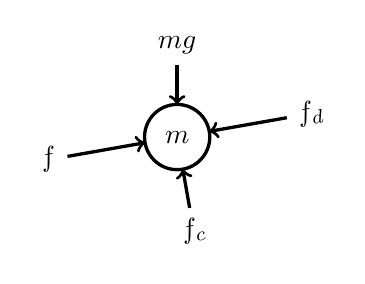
\begin{tikzpicture}[very thick,
sysblock/.style={draw,rectangle,inner sep=6pt,minimum width=1.5cm,minimum height=1.2cm,very thick},
delayblock/.style={draw,rectangle,inner sep=6pt,minimum width=0.5cm,minimum height=1.0cm,very thick},
node/.style={fill,inner sep=0pt,outer sep=0pt},
summer/.style={circle,draw,very thick,inner sep=5pt,outer sep=0pt}]

\draw (0,0) node[summer] (M1) {$m$};

%\draw[thin]  (M1.-90) -- ++(2,0);
%\draw (M1.-90) ++(6:1.5) node {$\phi$};
%\draw[|->] (M1.-90) ++(0,-1) -- ++(1,0) node[right] {$x$};
\draw[->] (M1.190) ++(10:-1) node[rotate=10,left] {$f$} -- (M1.190);
\draw[->] (M1.90) ++(0,0.5) node[above] {$mg$} -- ++(0,-0.5);
\draw[->] (M1.-80) ++(-80:0.5) node[rotate=10,below] {$f_{c}$} -- (M1.-80);
\draw[->] (M1.10) ++(10:1) node[rotate=10,right] {$f_d$} -- (M1.10);

\end{tikzpicture}

\end{center}
%\caption{Balancing Two Wheeled Robot}\label{fig:two wheeled}
%\end{figure}
We assume that the robot is always in contact with the road, and thus the position along the $y$ axis is always $r(x)$. Newton's law in the $x$ and $y$ axes gives the following:
\begin{align*}
 {\mbox{acceleration in $y$ axis}} \quad\ m\ddot{y} &= f_{c}\cos(\phi) - mg + (f-f_{d})\sin(\phi)  \\
 {\mbox{acceleration in $x$ axis}} \quad m\ddot{x} &= (f-f_{d})\cos(\phi) - f_{c}\sin(\phi) 
\end{align*}
Since the movement along the $y$ axis is prescribed by the road, we have $y=r(x)$ and
\begin{align*}
\dot y &= \frac{dr}{dx}\dot{x}\\
\ddot y &= \frac{d^2r}{dx^{2}}(\dot{x})^2+\frac{dr}{dx}\ddot{x}.
\end{align*}
We plug this into the first equation, multiply by $\sin(\phi)$ and multiply the second equation by $\cos(\phi)$. 
\begin{align*}
m\left(\frac{d^2r}{dx^{2}}(\dot{x})^2+\frac{dr}{dx}\ddot{x}\right)\sin(\phi) &= f_{c}\cos(\phi)\sin(\phi) - mg\sin(\phi) + (f-f_{d})\sin^2(\phi) \\
m\ddot{x}\cos(\phi) &= (f-f_{d})\cos^2(\phi)- f_{c}\sin(\phi)\cos(\phi) 
\end{align*}
By adding the two equations, we eliminate $f_{c}$
\[
m\left(\frac{d^2r}{dx^{2}}(\dot{x})^2\sin(\phi)+\frac{dr}{dx}\ddot{x}\sin(\phi) + \ddot{x}\cos(\phi)\right) =  - mg\sin(\phi) + (f-f_{d})(\cos^{2}(\phi) +\sin^2(\phi)) 
\]
Solving for $\ddot{x}$ and simplifying (using $\sin^{2}(\phi) + \cos^2(\phi)=1$),
\[
\ddot{x} = \frac{1}{\frac{dr}{dx}\sin(\phi) + \cos(\phi)}\left[ -\frac{d^2r}{dx^{2}}(\dot{x})^2\sin(\phi) - g\sin(\phi) + \frac{1}{m}(f-f_{d})\right] 
\]
Now, the damping force is given by $f_{d} = b\dot{v}$. Since the car moves along the road, the velocity $v$ is given by  $\dot{v}=\frac{\dot{x}}{\cos(\phi)}$, so that $f_{d} = \frac{b}{\cos{\phi}}\dot{x}$.
Some further simplification is possible since the slope $\frac{dr}{dx}$ and the angle $\phi$ are related. In fact, $\tan(\phi) = \frac{dr}{dx}$. Then
\begin{align*}
\frac{dr}{dx}\sin(\phi) + \cos(\phi) &= \tan(\phi)\sin(\phi) + \cos(\phi) \\
& = \frac{\sin(\phi)}{\cos(\phi)}\sin(\phi) + \cos(\phi) \\
& = \frac{\sin^2(\phi) + \cos^2(\phi)}{\cos(\phi)}\\
& = \frac{1}{\cos(\phi)}
\end{align*}
and our final equation is 
\[
\ddot{x} = \cos(\phi)\left[ -\frac{d^2r}{dx^{2}}(\dot{x})^2\sin(\phi) - g\sin(\phi) + \frac{1}{m}f - \frac{b}{m\cos(\phi)}\dot{x}\right] 
\]


\end{document}


